\documentclass[../main.tex]{subfiles}

% 4.1.1 Figuren
\begin{figure}[ht]
    \centering
        \begin{subfigure}[b]{0.4\textwidth}
            \begin{tikzpicture}
                \node[anchor=south west,inner sep=0] (image) at (0,0) {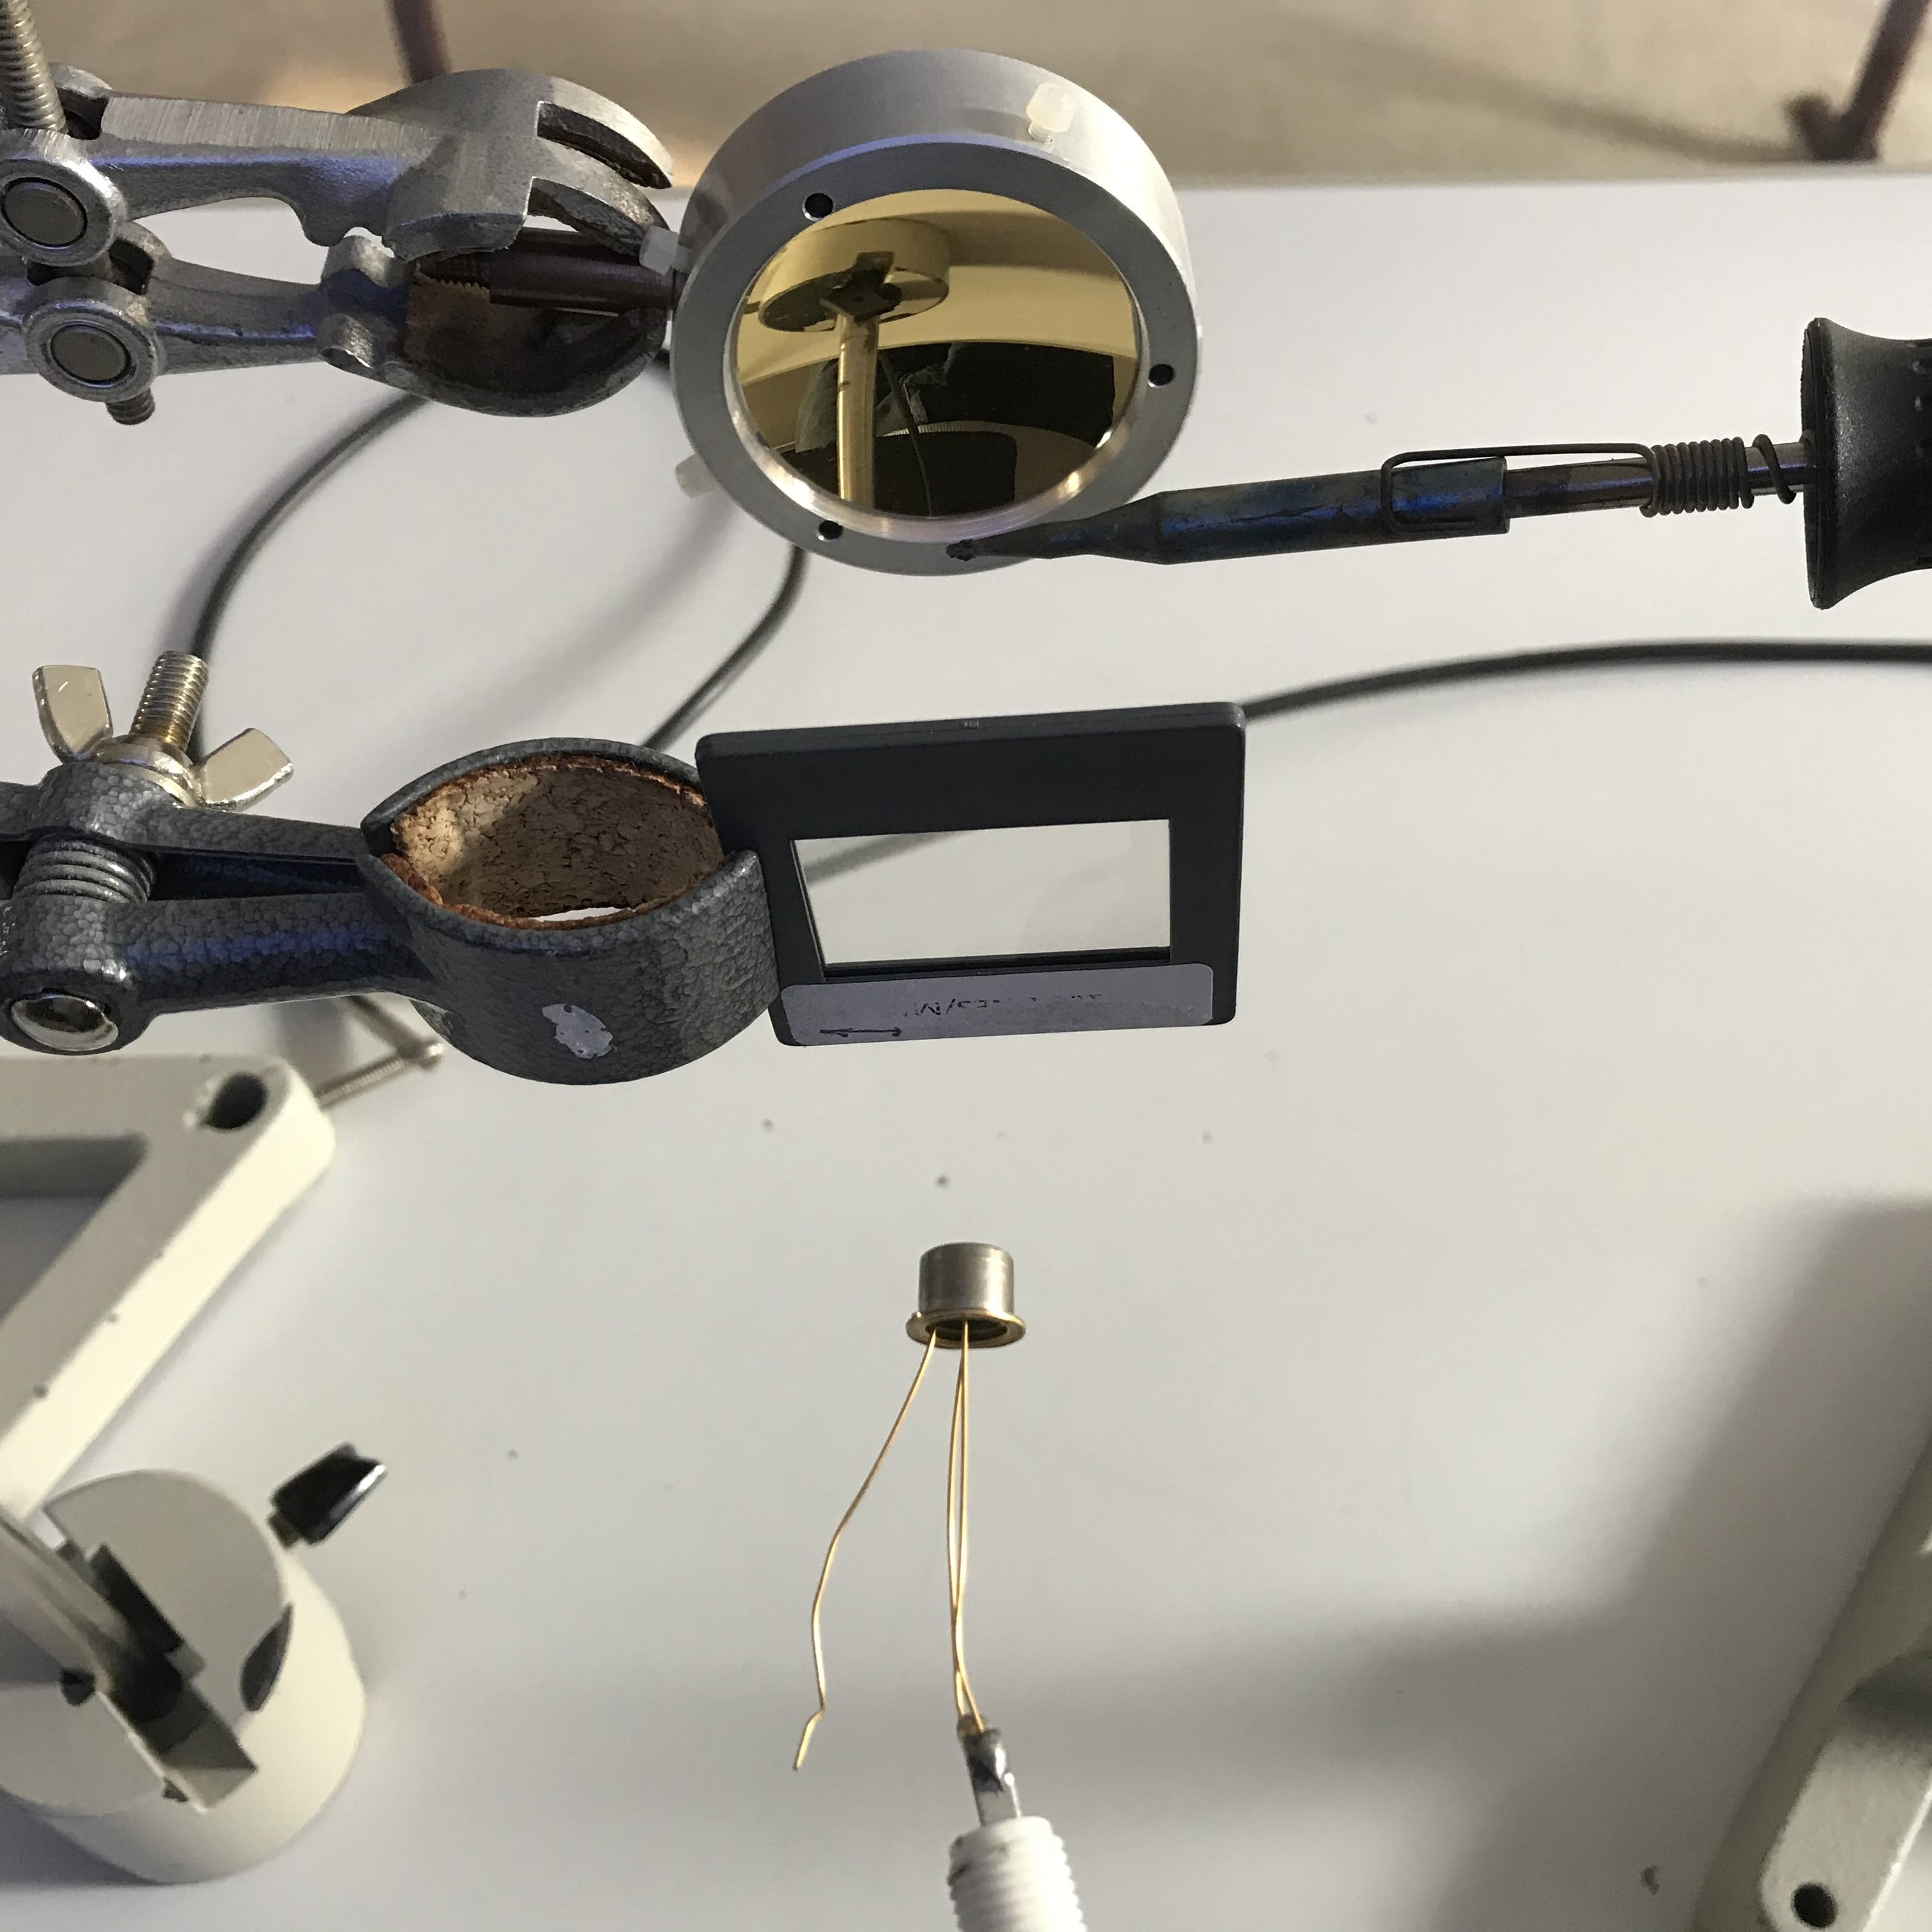
\includegraphics[width=\textwidth]{experiment/spektrometer-aufbau-frontal.jpg}};
                \begin{scope}[x={(image.south east)},y={(image.north west)}]
                    \draw (0.75,0.85) node[fill=white] {Spiegel};
                    \draw (0.3,0.7) node[fill=white] {Lötkolben};
                    \draw (0.8,0.55) node[fill=white] {Gitter};
                    \draw (0.7,0.3) node[fill=white] {Sensor};
                \end{scope}
            \end{tikzpicture}
        \end{subfigure}
        \begin{subfigure}[b]{0.4\textwidth}
            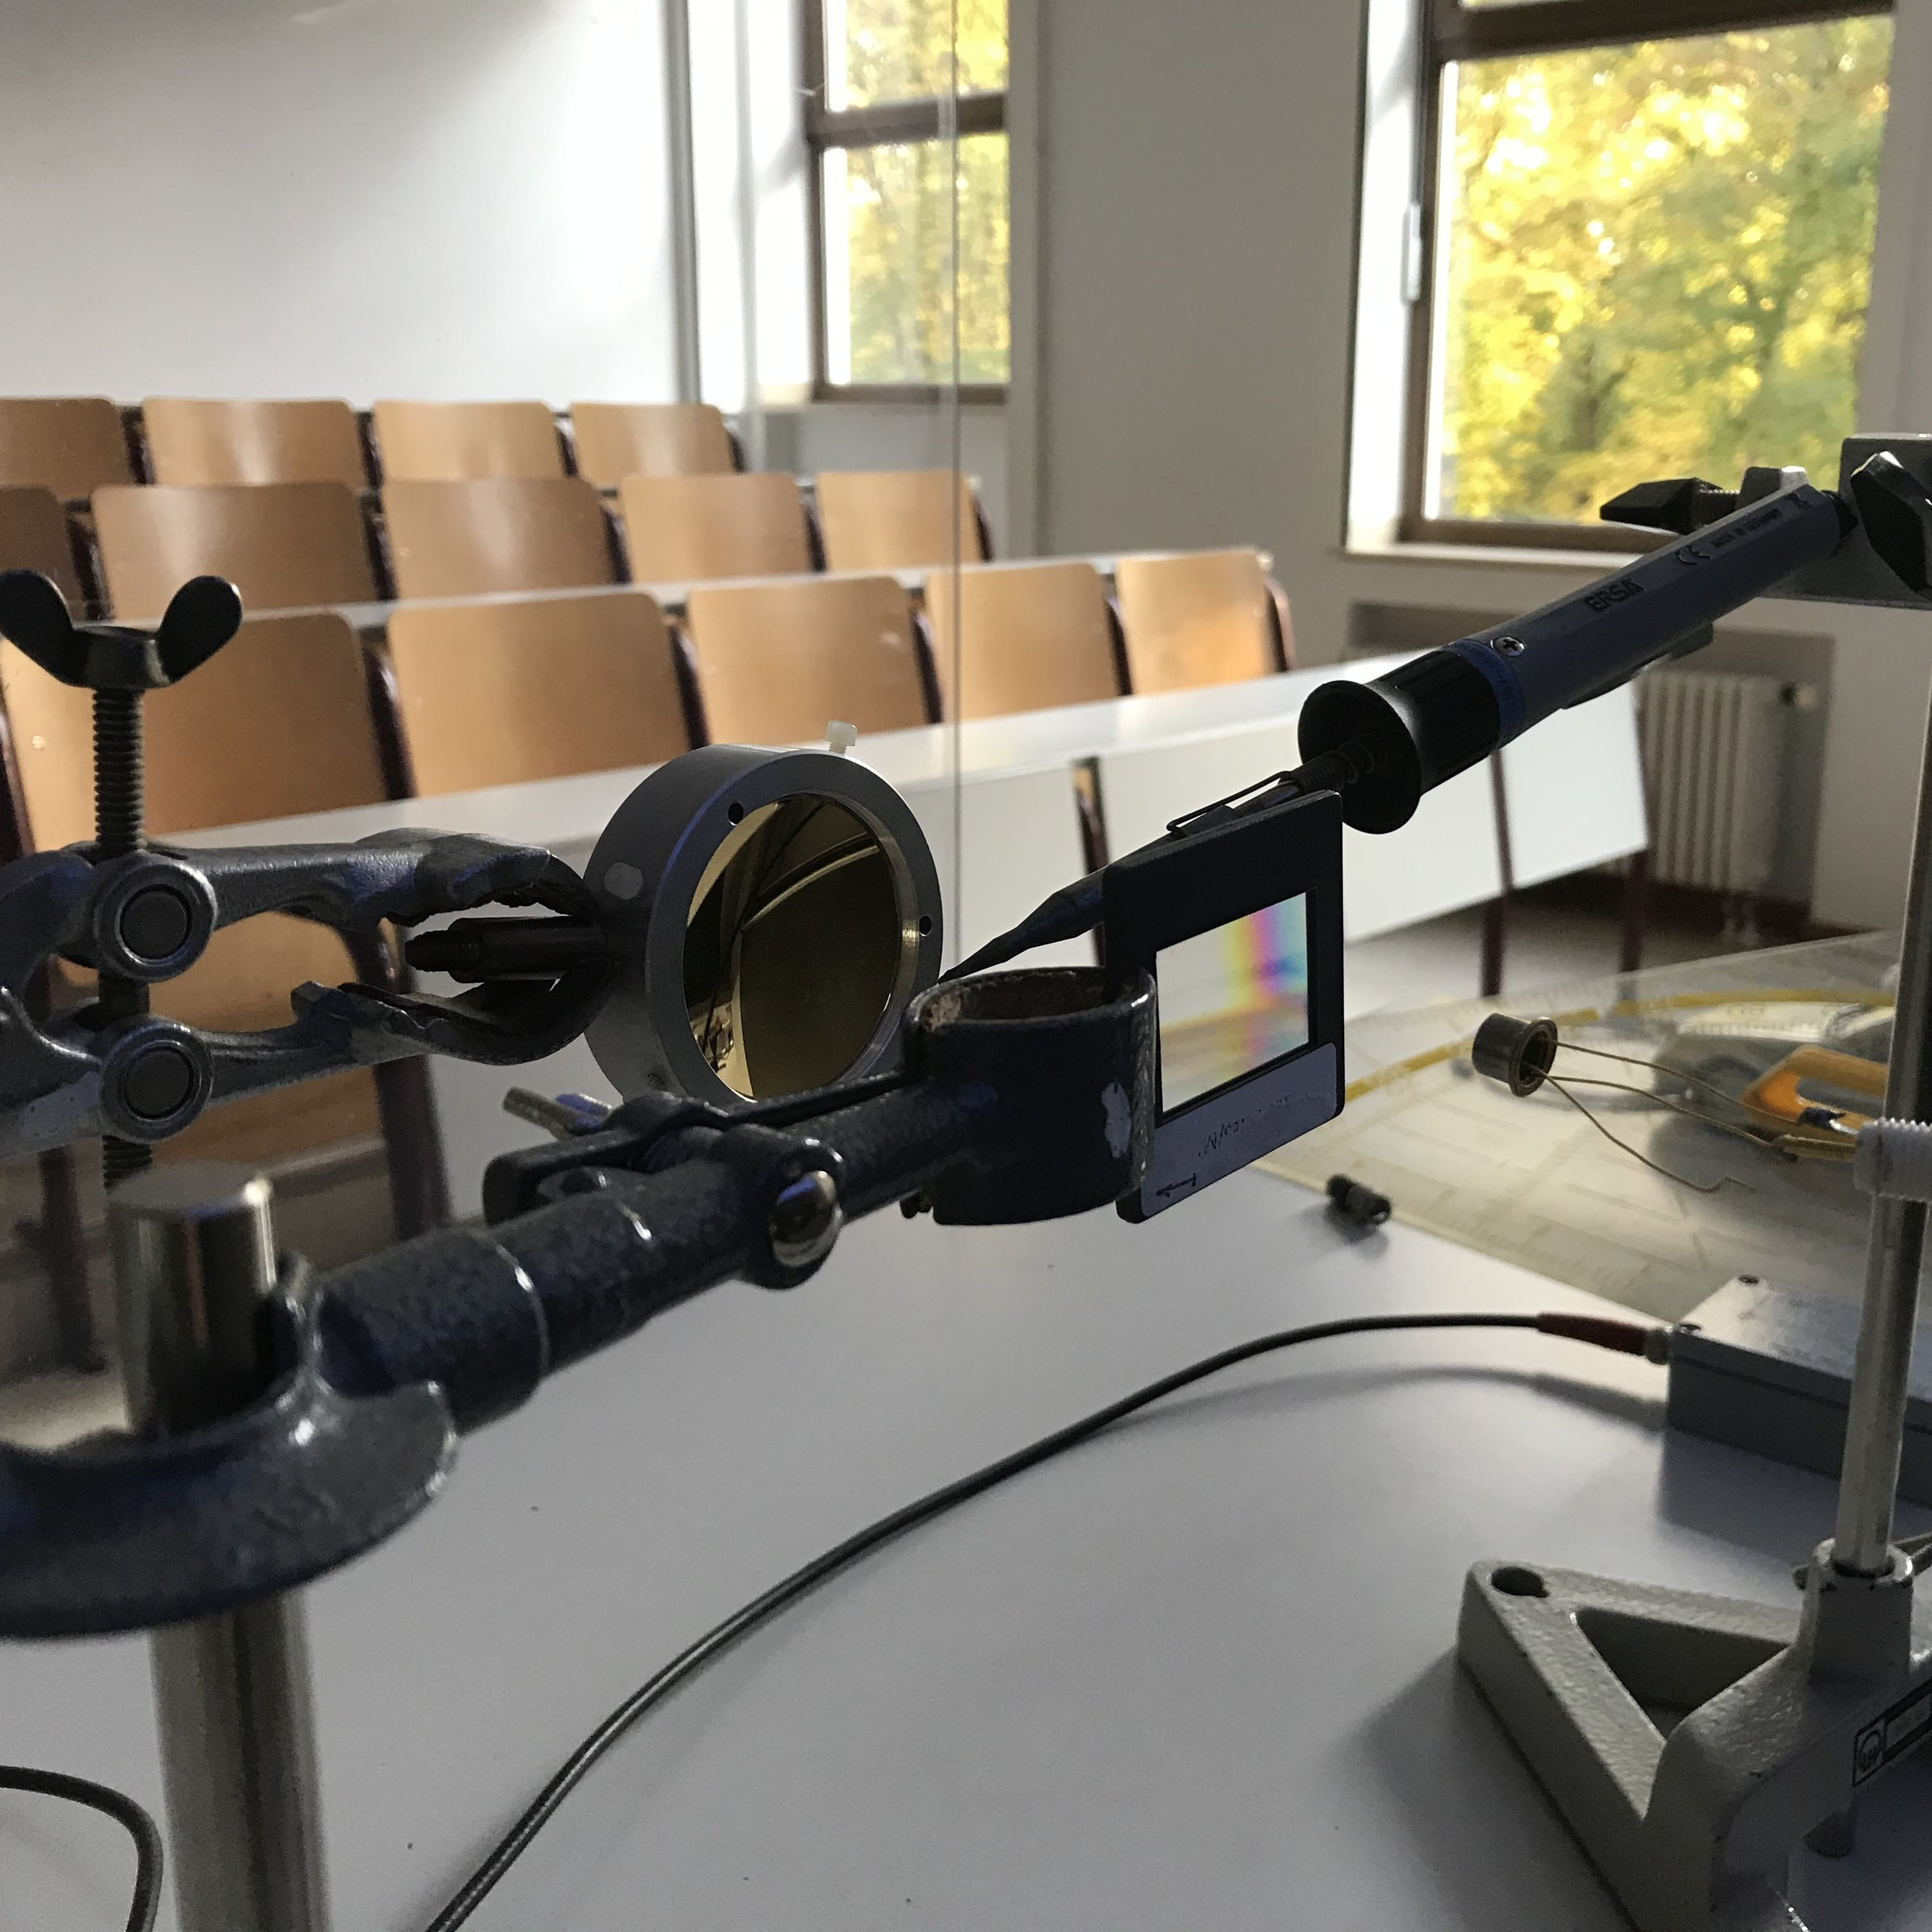
\includegraphics[width=\textwidth]{experiment/spektrometer-aufbau-seitlich.jpg}
        \end{subfigure}
        \caption{Versuchsaufbau; von hinten nach vorne: Vergoldeter Parabolspiegel, Lötkolben, Gitter mit 100 Linien/mm, hochempfindliche Thermosäule.}
\end{figure}

\begin{figure}[ht]
    \centering
        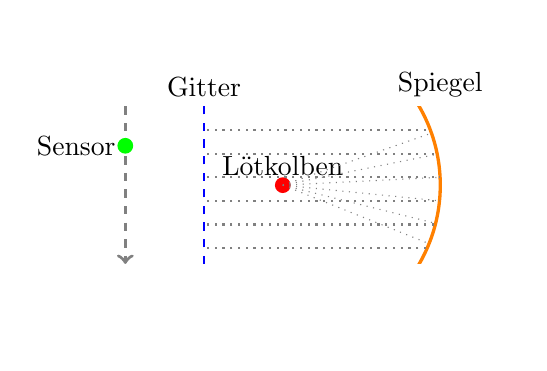
\begin{tikzpicture}
            % Spiegel
            \begin{scope}
                \clip (2,1) rectangle (4,-1);
                \draw (1,0)[orange,very thick] circle (2);
            \end{scope}
            \draw (3,1) node[black,anchor=south] {Spiegel};
            
            \fill[red] (1,0) circle (0.1) node[black,anchor=south] {Lötkolben};
            
            % EM-Strahlungen
            \begin{scope}
                \clip (1,0) circle (2);
                \clip (0,-1) rectangle (3,1);
                \foreach \i in {0.3,0.6,...,2} {
                    \draw[gray,dotted] (1,0) -- (3,{\i-1.1}); % Abgegeben
                    \draw[gray,dotted,thick] (4,{\i-1.1}) -- (0,{\i-1.1}); % Reflektiert
                }
            \end{scope}
            
            \draw[blue,thick,dashed] (0,-1) -- (0,1) node[black,anchor=south] {Gitter};
            
            \draw[very thick,gray,dashed,->] (-1,1) -- (-1,-1);
            \fill[green] (-1,0.5) circle (0.1cm) node[black,anchor=east] {Sensor};
        \end{tikzpicture}
    \caption{Schematischer Versuchsaufbau}
    \label{fig:versuchsaufbau-schematisch}
\end{figure}

Der Aufbau ist wie folgt (Abb. \ref{fig:versuchsaufbau-schematisch}): Ein Lötkolben gibt eine punktförmige Infrarotstrahlung ab, welcher vom Spiegel als Parallelstrahl zum Gitter reflektiert wird. Die gebeugten Wellen werden vom Sensor dedektiert.
